% !TeX program = xelatex
% 与所提供电赛模板使用相同的 ctexart / XeLaTeX 环境。
\documentclass[UTF8,zihao=5,fontset=none]{ctexart}
\linespread{1}
\usepackage{geometry,graphicx,amsmath,amssymb,float,hyperref,listings,xcolor,booktabs,fancyhdr}
\usepackage{multicol,caption,array}
% 优先沿用电赛模板的思源字体；未安装时自动使用 TeX 发行版自带字体。
\IfFontExistsTF{Source Han Serif SC}{\setCJKmainfont{Source Han Serif SC}}{\setCJKmainfont{FandolSong-Regular.otf}[BoldFont=FandolSong-Bold.otf,ItalicFont=FandolKai-Regular.otf]}
\IfFontExistsTF{Source Han Sans SC}{\setCJKsansfont{Source Han Sans SC}\setCJKmonofont{Source Han Sans SC}}{\setCJKsansfont{FandolHei-Regular.otf}[BoldFont=FandolHei-Bold.otf]\setCJKmonofont{FandolFang-Regular.otf}}
\IfFontExistsTF{Times New Roman}{\setmainfont{Times New Roman}}{\setmainfont{TeX Gyre Termes}}
\setCJKfamilyfont{kai}{FandolKai-Regular.otf}
\geometry{a4paper,left=1.5cm,right=1.5cm,top=2.5cm,bottom=1.5cm,footskip=.85cm}
\setlength{\columnsep}{.75cm}
\setlength{\parindent}{2em}
\setlength{\parskip}{1.5pt}
\setlength{\multicolsep}{8pt}
\pagestyle{fancy}\fancyhf{}\renewcommand{\headrulewidth}{0pt}\cfoot{\fontsize{9}{11}\selectfont\thepage}
\hypersetup{hidelinks,pdftitle={水下作业机器人系统设计与任务实现},pdfauthor={某某队}}
\ctexset{section={format=\sffamily\fontsize{12}{16}\selectfont,beforeskip=7pt,afterskip=3pt,number=\arabic{section}},subsection={format=\normalfont\fontsize{10.5}{15}\selectfont,beforeskip=5pt,afterskip=3pt}}
\setcounter{section}{-1}
\DeclareCaptionFont{reportcaption}{\sffamily\fontsize{9}{12}\selectfont}
\captionsetup{font=reportcaption,labelsep=space,skip=4pt,hypcap=false}
\graphicspath{{pic/}}
\setlength{\emergencystretch}{1em}
\begin{document}
\begin{center}
{\sffamily\fontsize{16}{21}\selectfont 水下作业机器人系统设计与任务实现\par}
\vspace{6pt}
{\fontsize{9}{12}\selectfont 某某队\par （上海海事大学，上海）\par}
\end{center}
{\CJKfamily{kai}\fontsize{9}{13}\selectfont\noindent 摘要：针对水下作业赛中的探测器开启、矿石收集和风电机组维护任务，设计一套采用八推进器布局的有缆水下作业机器人方案。系统以现有机器人本体为安装基础，将大范围定位交给载体运动，前端配置两指夹爪、受限旋转腕和可换接触件，分别适应拔取、插接、球体抓取及线缆挂装。结合道具形态，对承力路径、质量控制、浮力配平、作业视野和低速操作进行设计，并给出任务实施顺序与故障处置方法。分析表明，旋钮超过180\(^{\circ}\)的有效行程、锌块分步拆装以及护套挂装时的线缆稳定性，是末端设计需要重点满足的条件。采用主相机观察、定航定深辅助与短时点动相结合的方式，为近场操作提供控制方案；通过单项重复试验和600 s综合演练评价任务表现，为后续确定机构尺寸和控制参数提供依据。\par\noindent 关键词：水下机器人；水下作业；末端执行器；矢量推进；遥操作\par}
{\fontsize{9}{12}\selectfont\noindent 中图分类号：TP242\quad 文献标识码：A\par}
\begin{center}
{\fontsize{14}{18}\selectfont System Design and Task Execution of an Underwater ROV\par}
\smallskip{\fontsize{9}{12}\selectfont Team Name\par (Shanghai Maritime University, Shanghai, China)\par}
\end{center}
{\fontsize{9}{12}\selectfont\noindent Abstract: This paper presents a tethered underwater robot design for detector activation, mineral collection, and wind turbine maintenance tasks. An existing eight-thruster vehicle provides the mounting platform and performs large-scale positioning. A two-finger gripper, a limited-rotation wrist, and interchangeable contact pieces are proposed for extraction, insertion, spherical-object grasping, and cable handling. The design addresses load transfer, mass control, buoyancy trimming, visual access, and low-speed operation. Task sequences and fault responses are developed for the competition environment. The analysis identifies effective rotation beyond 180 degrees, staged zinc-block removal, and cable stability during sleeve installation as important requirements for the end-effector. Camera observation, assisted heading and depth control, and short motion commands are combined to support close-range manipulation. Repeated individual-task tests and 600-second integrated trials are specified to evaluate performance and guide the selection of mechanical dimensions and control parameters.\par\noindent Keywords: underwater robot; underwater operation; end-effector; vectored propulsion; teleoperation\par}
\fontsize{10.5}{17}\selectfont
\begin{multicols}{2}
\raggedcolumns
\section{引言}

水下作业赛将海底探测器开启、矿石收集和海洋装备维护集中在同一场比赛中。操作手只能观察机器人回传画面，需要在10 min内完成拔取、插接、旋转和挂装等操作\textsuperscript{[1]}。与单纯航行相比，这些任务更容易暴露近场视野、低速姿态控制和末端接触方面的问题：夹爪虽然已经靠近目标，却可能因视差对不准接口；旋转机构开始施力后，机体又可能随反力偏转。\par

水下机械臂的结构、驱动方式及控制方法需要与载体能力共同考虑\textsuperscript{[2]}。对于小型ROV，增加关节能够扩大操作范围，也会带来增重、密封和维护问题。已有六自由度ROV的研制工作表明，机械、电气与软件的协调设计是完成水下任务的重要基础\textsuperscript{[3]}。结合比赛道具和现有八推进器本体，我们将设计重点放在前端作业机构、浮力配平、操作视野与动作顺序上，由机器人本体完成大范围定位，由夹爪和旋转腕完成接触操作。\par

\columnbreak
\section{任务需求与总体方案}

\subsection{设计约束}

比赛要求机器人采用有缆遥控水下机器人（ROV）形态，质量不超过20 kg，不含脐带缆；机械手闭合后能够完全放入2 m\(\times\)1 m\(\times\)1 m空间，脐带缆长度不小于15 m。推进动力来自水下推进器，螺旋桨外应配置导流罩\textsuperscript{[1]}。这些条件首先限制了附件的数量和布置方式。机械手、支架、配重与相机均计入参赛配置，不能在本体完成后再无约束地叠加。\par

表1列出比赛的质量、包络和缆长限制，以及本方案的推进和末端配置。方案以紧凑框架和前置作业区为基础，控制夹爪收拢后的外形尺寸。脐带从机体上后方引出，既避开作业区，也便于拖缆手观察缆线状态。\par

\begin{center}\begin{minipage}{\linewidth}\centering\captionof{table}{竞赛约束与方案指标}\smallskip{\setlength{\tabcolsep}{3pt}\renewcommand{\arraystretch}{1.25}\begin{tabular}{>{\centering\arraybackslash}p{.425\linewidth}>{\centering\arraybackslash}p{.515\linewidth}}\toprule

\textbf{项目} & \textbf{要求} \\\midrule

整机质量m/kg & \(\leq\)20，不含脐带缆 \\

闭合包络L\(\times\)W\(\times\)H/m & \(\leq\)2\(\times\)1\(\times\)1 \\

脐带长度l/m & \(\geq\)15 \\

推进方案 & 4台水平、4台垂向，配导流罩 \\

末端设计 & 夹持、释放及绕夹持轴线旋转 \\

腕部设计行程 & 支持90\(^{\circ}\)定位及超过180\(^{\circ}\)的操作 \\

\bottomrule\end{tabular}}\end{minipage}\end{center}

\subsection{任务分解}

任务A需要先释放并安放水听器，再完成插头连接和开关操作；任务B要求把球形矿石放入收集框；任务C包括线缆架设、护套挂装和锌块更换。三类任务都需要夹持和转运，但接触条件不同。插接对轴线偏差敏感，球体抓取容易滑脱，柔性线缆则可能在运输和释放时缠绕或脱架。\par

因此，末端采用两指夹爪与旋转腕组合。夹爪接触件兼顾柱状件和球形件，辅助挂钩负责引导线缆和护套。换装主要安排在训练和场间维护阶段，单场比赛尽量使用同一套末端件，减少上岸调整占用时间。视觉系统先利用主相机覆盖作业区，若夹爪遮挡无法通过安装位置解决，再增设近景视角。\par

\section{机械结构与推进系统}

\subsection{本体与安装布局}

机器人采用开放式框架，将密封舱、电池和主要质量集中在中部，浮力材料布置在上方，配重位于底部。图1为所用基础本体的结构示意\textsuperscript{[4]}。在这一安装基础上，前端作业板与主框架连接，机械手、相机和灯具分别设置安装基准，避免拆换接触件时改变相机与夹爪的相对位置。\par

\begin{center}\begin{minipage}{\linewidth}\centering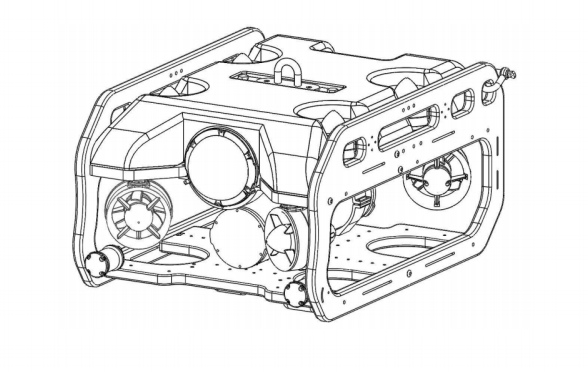
\includegraphics[width=.965\linewidth]{body.png}\captionof{figure}{机器人基础本体结构示意\textsuperscript{[4]}}\end{minipage}\end{center}

拔栓和旋转产生的反力由作业板传入主框架，不经过相机或灯具支架。前端机构尽量靠近纵向中心线，以减小偏心操作引起的艏摇力矩。夹爪全开、腕部转到极限位置时，接触件均应避开推进器和相机；挂钩在不使用时收于框架轮廓内，端部采用圆钝结构，减少挂缆和划伤道具的可能。\par

\subsection{八推进器布置}

四台水平推进器采用矢量布置，负责前后运动、横移和艏向调整；四台垂向推进器负责升沉，并通过前后或左右差动修正俯仰和横滚。图2给出功能布局。推进器方向、桨型和通道编号需一一对应，调试时先检查单台正反转，再检查整机运动，避免在混合输出下判断错误。\par

\begin{center}\begin{minipage}{\linewidth}\centering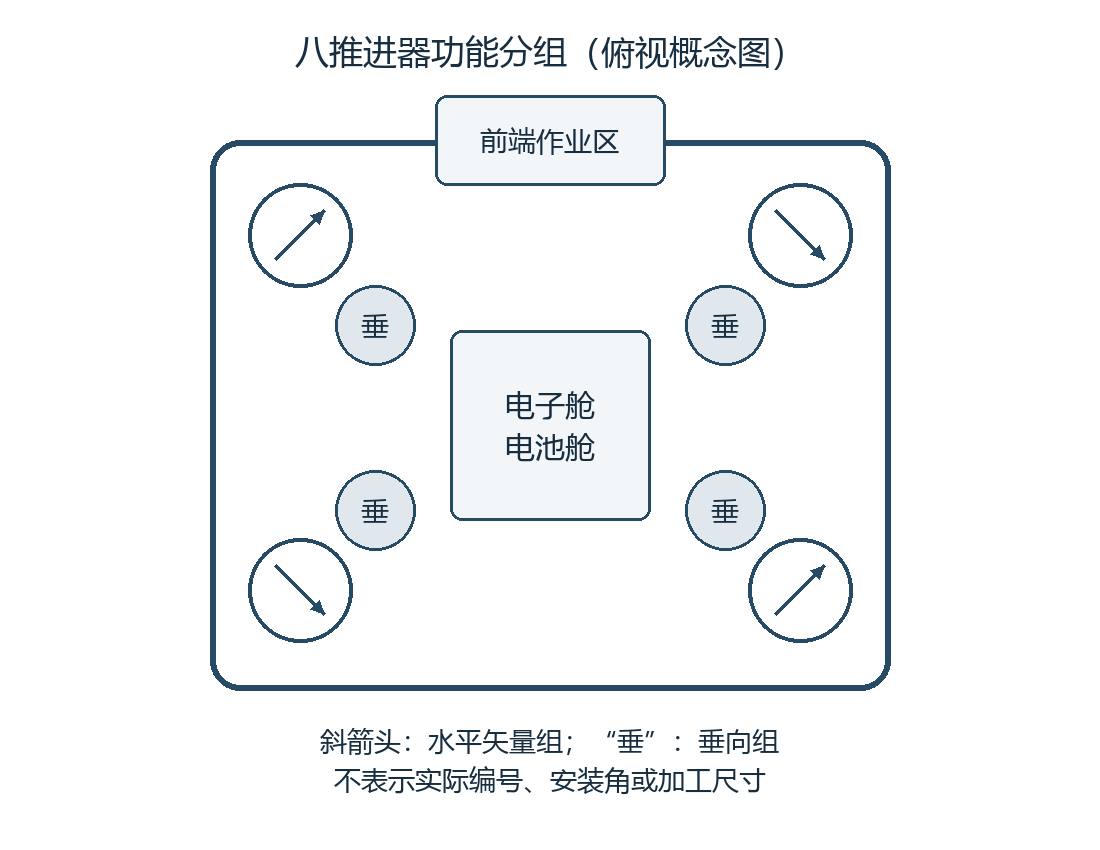
\includegraphics[width=.965\linewidth]{thrusters.png}\captionof{figure}{八推进器功能布局}\end{minipage}\end{center}

各推进器推力合成为机体的力和力矩，可表示为\par

\begin{equation}\boldsymbol{\tau}=\mathbf{B}\mathbf{f}\end{equation}

式中，\(\boldsymbol{\tau}\)为六维力与力矩向量，f为推进器推力向量，B由推进器方向和安装位置确定。实际输出还受电机死区、推力饱和与相互扰流影响，因而控制分配不能只依据几何关系。靠近目标时应降低输入增益，并分别观察横移、升沉和转向响应，寻找操作手能够稳定重复的小幅动作。\par

转场阶段可以使用较大的推力输出，接触前则应提前减速。插接时连续前推会把视觉延迟变成额外位移，也可能使夹爪抵住道具后继续施力。因此，近场操作采用短时点动，停稳观察间隙后再继续，而不靠提高推力强行纠正位置偏差。\par

\subsection{质量与浮力配平}

附件增加后，质量与浮力需要同时调整。质量核算按完整参赛状态进行，电池、支架、线束、夹爪、浮力材料和配重均纳入统计。新增模块采用轻量化支架和局部替换，优先减少冗余材料；推进器护罩和水密部件不作为减重对象。浮力材料能够改变水中受力，却不能抵消称重时增加的质量。\par

静水中的净浮力为\par

\begin{equation}F_{\text{净}}=\rho gV_{\text{排}}-mg\end{equation}

其中\(\rho\)为水密度，\(V_{\text{排}}\)为实际排水体积，m为总质量。开放框架的外包体积不能直接作为排水体积。以20 kg、淡水密度1 000 kg/m\textsuperscript{3}为例，中性浮力需要约20 L排水体积；若采用轻微正浮力，还需根据浮力材料自重增加适当排水量。这个计算用于确定配平方向，最终仍以水中姿态和浮沉趋势调整。\par

浮心位于重心上方时，机器人受扰后具有一定的姿态恢复能力。机械手伸出或抓取物体会使重心前移，因此底部配重保留前后调整位置。配平分别检查空载、安装完整作业机构和携带代表性道具三种状态。若夹持后明显低头，应先调整质量分布，减少依靠垂向推进器长期补偿的需求。\par

\subsection{脐带布置}

脐带固定在框架上，通过应力释放结构承担拉力，避免水密接插件直接受力。机体内部线束沿框架内侧敷设，不跨越夹爪运动区和推进器吸入口。转向过程中应留意缆线是否绕到机体前方，连续同向旋转尤其容易积累缠绕。\par

正式比赛中，拖缆手只负责收放缆线和避免缠绕，不主动牵引机器人，也不向操作手传递场地信息\textsuperscript{[1]}。训练时沿用同样的分工，才能检验任务是否确实依靠机载画面完成。若横移或转向受到持续缆力影响，应先调整走缆路径，避免单纯增大控制增益。\par

\section{作业机构与感知控制}

\subsection{旋转腕与夹爪}

前端机构按夹爪开合和腕部旋转两个主要动作进行设计，图3为结构方案。与长臂多关节方案相比，这种布置的悬臂较短，安装和密封较简单，适合由ROV本体承担定位的作业方式。其不足是不能在机体位置不变时大范围改变抓取方向，因此接近路线必须与工具轴线配合。\par

\begin{center}\begin{minipage}{\linewidth}\centering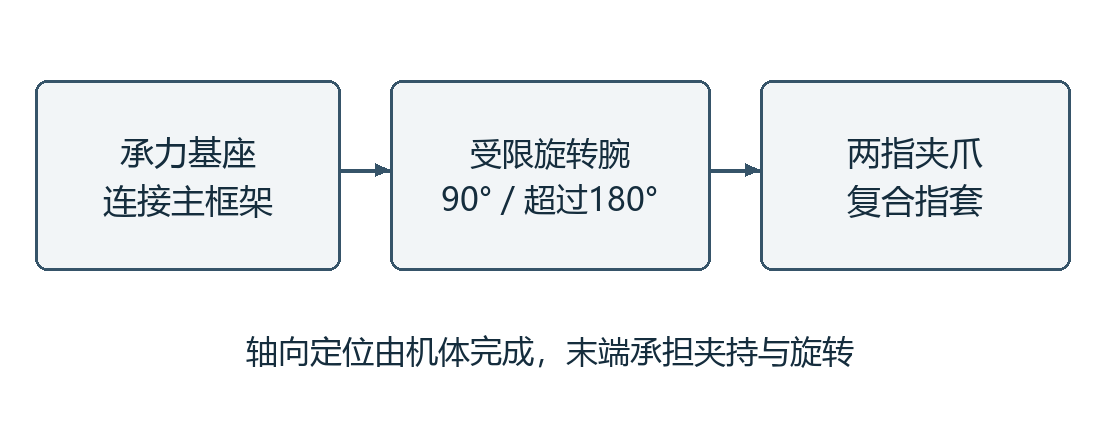
\includegraphics[width=.965\linewidth]{gripper.png}\captionof{figure}{旋转腕与末端执行器设计}\end{minipage}\end{center}

夹爪采用对称两指结构，接触件设置V形槽与弧形包络面。V形槽用于栓子和插头等柱状对象，弧面用于限制球形矿石滚动；接触表面配置耐水摩擦层，避免用光滑硬面直接挤压球体。规则中的矿石直径约42 mm，夹爪开口除容纳目标外，还应留出接近误差，但开口过大会增加闭合行程和对附近结构的干涉。\par

夹持能力同时取决于接触形状、夹紧力与湿态摩擦。对于两侧对称接触，若每侧法向力为N、摩擦系数为\(\mu\)，防滑条件可近似写为\par

\begin{equation}2\mu N\geq K F_{\text{载}}\end{equation}

式中，\(F_{\text{载}}\)为需要抵抗的等效外力，K为安全系数。栓子拔出和插头插入还包含接触阻力，不能仅按物体重量选取夹紧力。机构调试应检查湿态拉脱、行程限位和堵转保护，防止夹爪持续顶住道具或在运输途中松脱。\par

腕部行程由赛题决定。任务A要求旋钮实际转动超过180\(^{\circ}\)，因此180\(^{\circ}\)只能作为中间参考位置，不能设为有效行程终点。任务C拆旧锌块需要两次上提，每次配合90\(^{\circ}\)旋转；装新锌块也包含90\(^{\circ}\)旋转。腕部控制设计包含角度定位、回零和超时退出，线束按受限转角布置。机构命令角度与道具实际转角之间还可能存在回差和滑移，需要观察道具标记确认动作完成。\par

\subsection{作业视野与补光}

主相机布置在前上方，负责搜索、接近和观察夹爪。云台俯仰用于在航行视野与近场接触区之间切换；进入插接阶段后尽量固定相机角度，让操作手根据同一画面判断目标边缘、夹爪尖端及两者间隙。频繁调整云台会改变视觉参考，容易把镜头运动误认为机器人位移。\par

对于主相机看不到的接触面，可在作业板附近布置近景相机。新增相机不能遮挡夹爪或进入腕部包络，其价值取决于能否看清接口间隙，而不是视角数量本身。两路画面需要检查显示切换与延迟，避免操作手在不一致的视角之间反复判断。\par

补光灯放在相机两侧，光轴适当偏离镜头方向，减少金属道具表面的反光。近底水体受推进器扰动后可能出现悬沙，亮度过高反而会降低边缘对比度。照明调整应以看清目标为准，并在安装相机和工具后检查夹爪是否遮挡灯束。\par

\subsection{控制链路与模式选择}

系统由PC地面站、遥控手柄、通信中继、脐带缆和艇载控制单元组成，如图4所示。手柄输入和模式指令经通信链路下传，图像、深度、姿态及告警上传至地面站。推进、电气控制与作业机构分别管理，新增机械手驱动需配置支路保护，避免末端堵转影响控制电源。\par

\begin{center}\begin{minipage}{\linewidth}\centering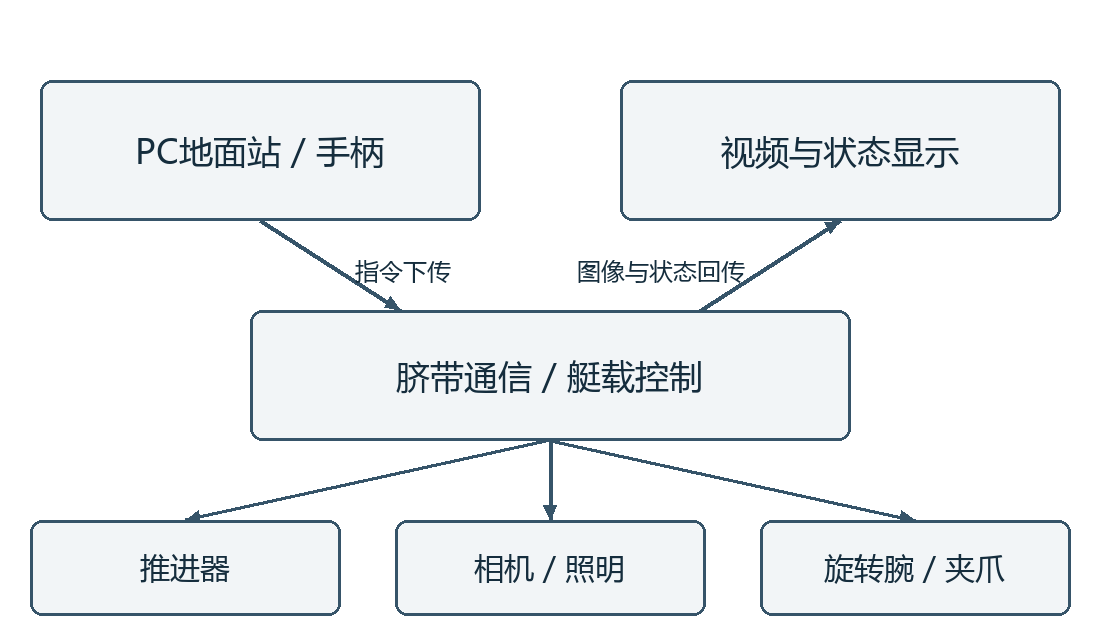
\includegraphics[width=.965\linewidth]{architecture.png}\captionof{figure}{地面操控与艇载系统连接}\end{minipage}\end{center}

地面站承担视频显示、参数设置和操作输入。定航模式用于辅助保持航向与姿态，定深模式增加深度保持；两者都不能直接替代水平位置控制。线缆拉力或作业反力仍可能使机器人平移，操作手需要根据画面修正位置。推进器安装位置、控制通道或传感器状态改变后，应重新检查方向映射和校准结果。\par

操作流程见图5。远距离接近采用手动模式，进入道具附近后降低增益，根据需要启用定航或定深。夹持后先做小幅试提或试转，确认没有误抓支架，再执行主要动作。目标滑脱、图像冻结或机构卡滞时，先停止继续施力，退出接触后重新对准。模式退出和锁定按键应保持明确，避免依赖多层菜单处理紧急情况。\par

\begin{center}\begin{minipage}{\linewidth}\centering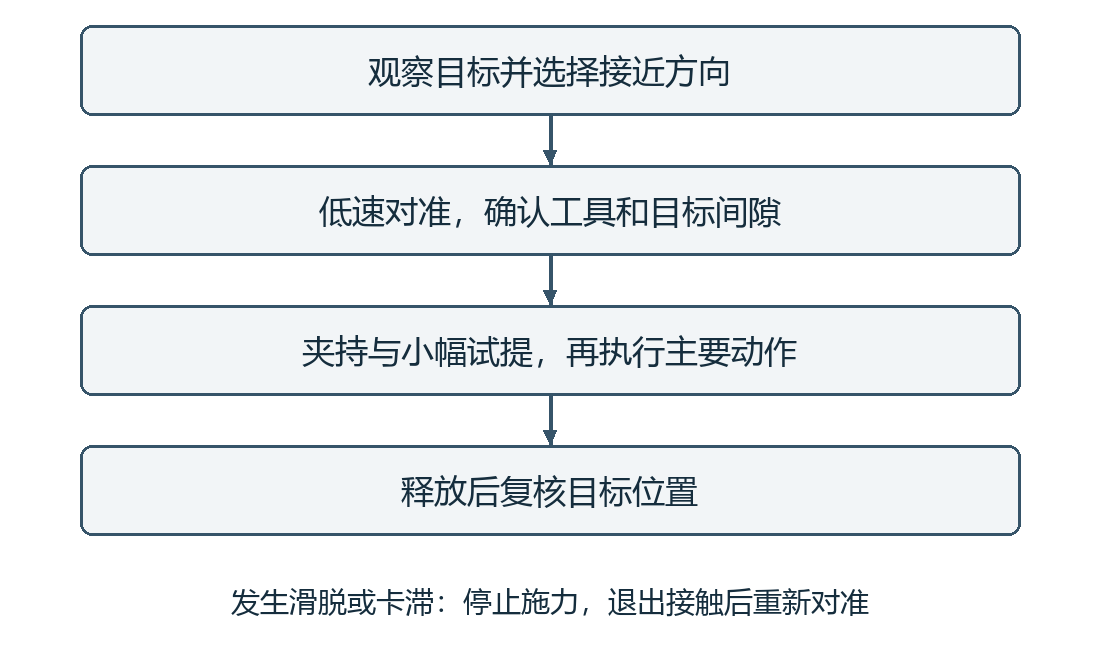
\includegraphics[width=.965\linewidth]{workflow.png}\captionof{figure}{近场作业操作流程}\end{minipage}\end{center}

\section{竞赛任务实施}

\subsection{海底探测器开启}

任务A的道具如图6所示。机器人首先接近电梯上的栓子，夹持后沿栓子轴向退出，减少侧向挤压。两个栓子解除后，取下水听器并运至安装处，释放后观察其是否稳定。随后移除连接箱对应上盖，取下插头，并使夹爪、插头与接口尽量位于同一轴线上。\par

\begin{center}\begin{minipage}{\linewidth}\centering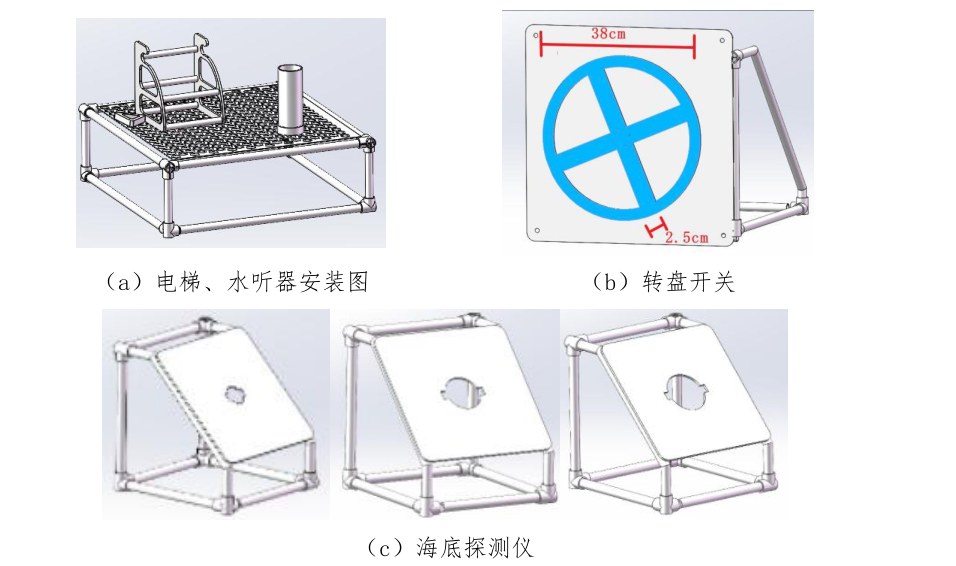
\includegraphics[width=.965\linewidth]{task_a.png}\captionof{figure}{任务A道具示意\textsuperscript{[1]}}\end{minipage}\end{center}

接口分为大、中、小三种，对应10、30、50分。选择小孔可以获得较高分值，但对准和重试耗时也可能增加。接近接口时先完成艏向调整，再用横移和升沉消除偏差，最后进行短距离轴向插入。若已经多次偏离且无法稳定对准，应结合剩余时间选择较大接口，不在单个动作上持续消耗比赛时间。\par

旋钮操作安排在连接完成后。夹爪应夹紧受力部位，腕部转动时观察机体是否偏转；必要时减小旋转速度并修正姿态，防止工具滑移。以道具实际转角超过180\(^{\circ}\)作为完成依据，释放后再次确认。任务A的得分按已完成的动作计算，三个孔径的插接分值不能累加。\par

\subsection{矿石收集}

任务B采用由近及远的搜索路线，先处理视野清楚、便于转运的目标。接近矿石时降低高度和速度，让球体进入夹爪包络后闭合，再小幅抬升确认夹持。运输过程中避免急转和快速升沉，防止惯性扰动使球体从接触面滑出。\par

收集框侧面和顶部设有约200 mm\(\times\)200 mm开口。末端进入投放位置即可，无需让机体整体穿过开口。侧向投放时应留意指套与框边间隙；顶部投放可减少横向穿孔的要求，但仍需观察释放后的落点。矿石准确进入框内才计20分，离开前应确认没有落在孔沿或被水流带出。任务B的矿石数量由现场决定，路线安排也应随目标分布调整。\par

\subsection{风电机组维护}

任务C包含线缆与锌块两部分，道具如图7所示。线缆从岸上接取后运到池底支架，先确认支撑点稳定，再收集护套。挂装时由短挂钩引导位置，夹爪避免大幅上提已经安放的线缆。6个护套分挂两端，每端最多计3个；若操作中使线缆整体或部分脱离支架，全部护套均不得分\textsuperscript{[1]}。\par

\begin{center}\begin{minipage}{\linewidth}\centering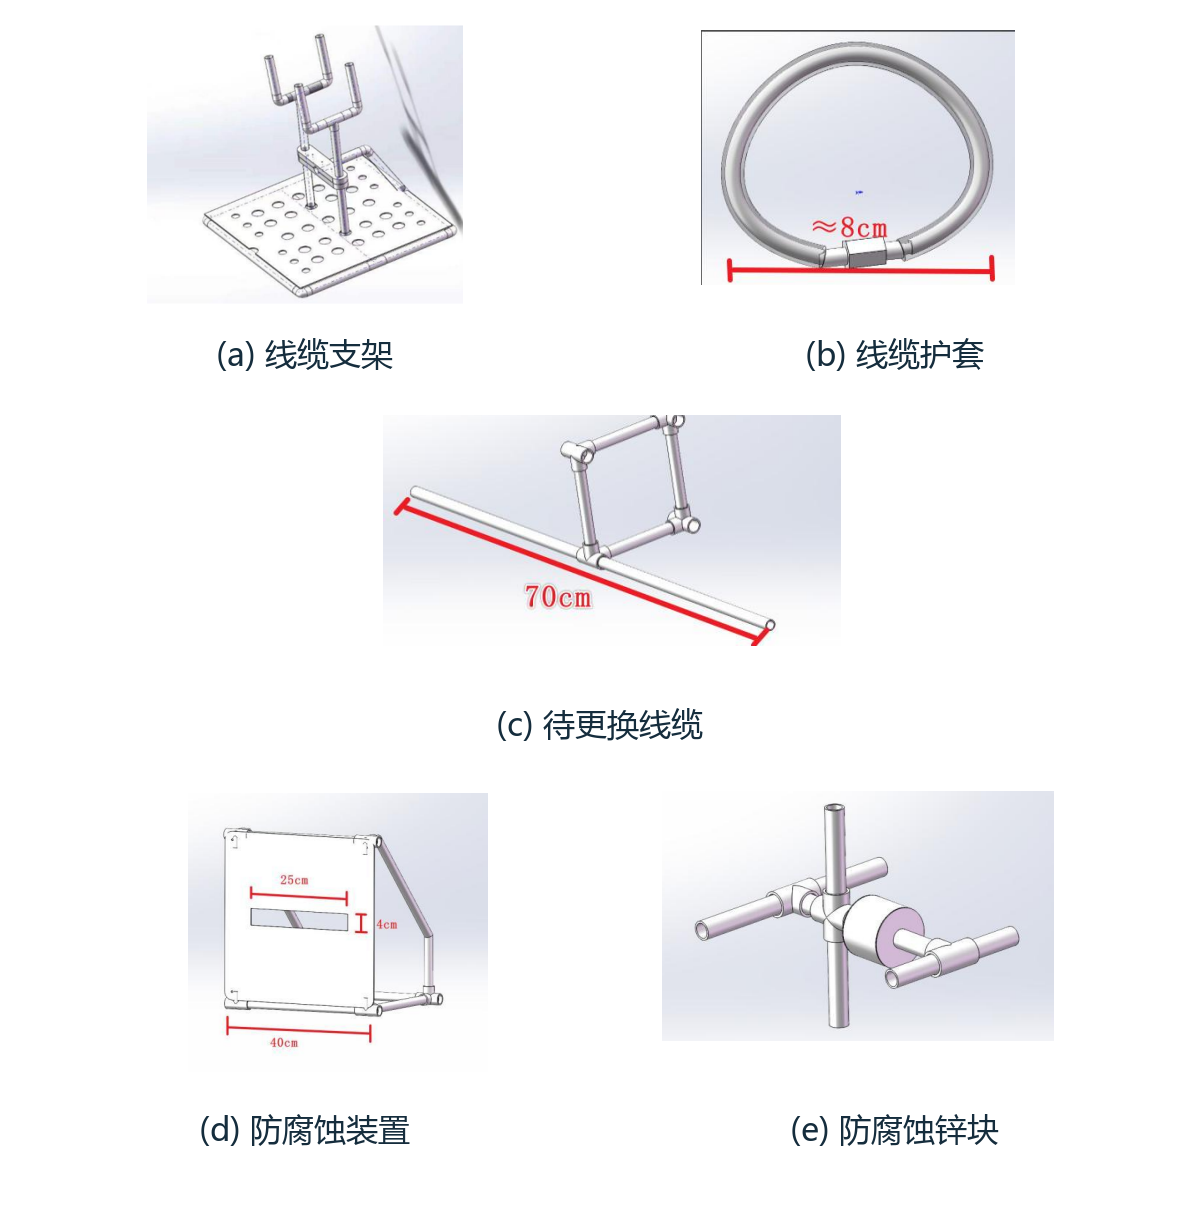
\includegraphics[width=.965\linewidth]{task_c.png}\captionof{figure}{任务C支架与维护道具\textsuperscript{[1]}}\end{minipage}\end{center}

旧锌块拆卸按卡槽逐级进行：先转动90\(^{\circ}\)并上提，通过一级约束后，再完成第二次90\(^{\circ}\)旋转与上提。旧块取下后送回出发区交给岸上队员，再接取新块返回安装，按安装方向完成90\(^{\circ}\)旋转。提、转和插入分步进行，可以减少卡槽受力不均造成的卡滞。\par

表2概括末端动作与控制方式的对应关系。正式比赛不固定采用一条航线，而是结合道具位置、往返距离和已完成任务选择下一步。线缆未放稳时不继续挂套；精细插接反复失败时，应避免挤占能够稳定完成的其他动作。\par

\begin{center}\begin{minipage}{\linewidth}\centering\captionof{table}{任务动作与实现方式}\smallskip{\setlength{\tabcolsep}{3pt}\renewcommand{\arraystretch}{1.25}\begin{tabular}{>{\centering\arraybackslash}p{.10\linewidth}>{\centering\arraybackslash}p{.39\linewidth}>{\centering\arraybackslash}p{.42\linewidth}}\toprule

\textbf{任务} & \textbf{主要动作} & \textbf{实现方式} \\\midrule

A & 拔栓、插接、开关旋转 & V形夹持、轴向点动、实际转角>180\(^{\circ}\) \\

B & 球体抓取与入框投放 & 弧面包络、低速转运、释放复核 \\

C & 线缆挂装与锌块更换 & 挂钩引导；旧块两轮90\(^{\circ}\)旋转与上提，新块90\(^{\circ}\)安装 \\

\bottomrule\end{tabular}}\end{minipage}\end{center}

任务得分以规则规定的过程和结束状态判定，不能把曾经完成的动作直接视为已经保分。提前完成全部任务后，机器人浮上水面并结束，剩余时间以分钟向下取整，每整分钟计10分。若尝试自主动作，需要在赛前向裁判说明，并明确体现机器人脱离操作手控制；定航、定深等辅助功能本身不等于获得自主动作双倍分。\par

\section{可靠性与试验安排}

\subsection{水密与供电}

电子舱、电池舱和执行器连接处是水密检查的重点。装配前清洁密封面，检查O形圈压痕、颗粒和扭转，恢复端盖与穿舱连接后再进行检漏。浅水作业并不能消除开舱复装和接插件受力造成的渗漏，任何涉及密封边界的改动都应重新检查。\par

电源按推进、控制传感、视觉照明和机械手分配负载。动力线与弱信号线分开固定，机械手支路考虑堵转电流，电池检查同时关注电压和负载下的压降。低电量告警应保留回收余量，不能仅凭容量或标称续航判断可以连续完成多场比赛。上电前确认手柄中位、控制模式和锁定状态，处理桨叶或缠绕前先断开动力。\par

\subsection{故障处置与维护}

出现图像冻结时停止盲操作，检查通信和地面端状态；夹爪卡滞时停止施力并尝试退出接触，避免继续夹紧损伤道具。漏水或持续低压报警时中止任务并尽快回收；通信丢失则依赖事先验证的失效保护。轻微正浮力有助于在未缠绕条件下上浮，但不能作为任何故障均能自动回收的保证。\par

经裁判允许后可以将机器人取出维修，维修期间计时继续，恢复后从出发区重新入水。场间维护以外部检查和已准备好的部件更换为主，复杂开舱和参数重置应在比赛前完成。出水后用清水冲洗框架和推进器，检查接触件磨损与密封状态，干燥后整理脐带和接插件，记录更换部件引起的质量与配平变化。\par

\subsection{试验方法与评价}

试验先从完整配置的质量、闭合尺寸、线缆长度和防护结构开始，再进行检漏、浅水静置和配平。基础运动测试逐项检查前后、横移、升沉与转向，确认模式切换和退出正常后，才进入接触作业。每轮固定结构、配重和参数，记录水深、照明、缆线状态以及操作手，减少条件变化对结果的影响。\par

单项试验围绕最容易失败的动作展开：插接观察轴线偏差和重试次数，矿石抓取记录滑脱与投放落点，旋钮和锌块操作检查实际转角、机体摆动及卡滞。比较不同指套或视角时，尽量保持其他条件一致，并交替安排测试顺序，避免把操作熟练度提高误认为机构改进。\par

成功率按成功次数与总尝试次数之比计算，完成时间从统一起点计时；失败、超时和人工纠正单独保留。综合试验按600 s进行，依据终场状态评分，同时记录护套挂装中的脱架事件。现阶段尚未形成同一配置下的完整重复试验数据，任务成功率和耗时不作量化结论，后续通过连续视频与操作记录验证方案。\par

\section{结束语}

本文围绕水下作业赛完成了八推进器本体与前端作业机构的配合设计。大范围定位由机体完成，两指夹爪和受限旋转腕承担抓取、插接及旋转。浮力和配重调整、固定近场视觉参考以及接触阶段降低输入增益，均以减小机体漂移和目标滑脱风险为目的，其效果需通过任务试验确认。\par

方案的重点在于使工具、视野和动作顺序相互配合。下一步需集中验证超过180\(^{\circ}\)旋钮操作、锌块分级拆装以及线缆护套挂装，结合重复试验确定指套几何、腕部输出和低速控制参数。最终参赛配置还应完成整机称重、水密与综合任务检验。\par

\section*{参考文献}

{\fontsize{9}{12}\selectfont\noindent\hangindent=1.5em\hangafter=1 [1] 某水下机器人竞赛组委会. 水下作业项目比赛规则及评审标准[R]. 示例规则，使用时替换.\par}\smallskip

{\fontsize{9}{12}\selectfont\noindent\hangindent=1.5em\hangafter=1 [2] Underwater manipulators: A review[J]. Ocean Engineering, 2018, 163: 431-450.\par}\smallskip

{\fontsize{9}{12}\selectfont\noindent\hangindent=1.5em\hangafter=1 [3] Design and Implementation of a Six-Degrees-of-Freedom Underwater Remotely Operated Vehicle[J]. Applied Sciences, 2023, 13(12): 6870.\par}\smallskip

{\fontsize{9}{12}\selectfont\noindent\hangindent=1.5em\hangafter=1 [4] SeaRobotix. FindROV H20 无人潜航器用户手册: V1.1[Z]. 2022-11.\par}\smallskip
\end{multicols}
\end{document}
